\section{\GJ v.s. Binary Join}

% \ds{This detailed description does not belong to the introduction;
%   here it suffices to say that \FJ outperforms traditional plans even
%   on cyclic queries, namely star queries.}  
% \ds{In fact your example
%   shows that \GJ is asympotitically faster than traditional plans even
%   on acyclic queries: explain $O(n)$ v.s. $O(n^2)$.  The reason is
%   that acylic queries do not implement Yannakakis faithfully.}
For an intuition of why \GJ may be faster than binary join, 
  consider the following query:
  \begin{lstlisting}[
    language=SQL,
    showspaces=false,
    basicstyle=\ttfamily\small,
    numbers=left,
    numberstyle=\tiny,
    commentstyle=\color{gray}
 ]
SELECT * FROM R, S, T -- schema: R(x,a), S(x,b), T(x,c)
 WHERE R.x = S.x AND S.x = T.x AND T.x = R.x
\end{lstlisting}
Note that this query is \emph{acyclic}.
A database instance for \texttt{R}, \texttt{S}, and \texttt{T} 
  is shown in Figure~\ref{fig:sand-dollar}.
We will refer to this query and database instance as the \emph{sand dollar query}.
There are only 4 values for the attribute $x$ in the database:
  $\set{x_0, x_1, x_2, x_3}$.
There are $2n+1$ values for each of $a$, $b$ and $c$:
  $\set{a_0, a_1^l, \ldots, a_n^l, a_1^r, \ldots, a_n^r}$, 
  and similar for $b$ and $c$. 
The relations $R$, $S$ and $T$ are as follows:
%
\begin{align*}
  R & = \set{(x_0, a_0)} \cup \bigcup_{i \in [1 \ldots n]} \set{(x_1, a_i^l), (x_2, a_i^r)} \\
  S & = \set{(x_0, b_0)} \cup \bigcup_{i \in [1 \ldots n]} \set{(x_2, b_i^l), (x_3, b_i^r)} \\
  T & = \set{(x_0, c_0)} \cup \bigcup_{i \in [1 \ldots n]} \set{(x_3, c_i^l), (x_1, c_i^r)} 
\end{align*}
%
It should be clear that the only output tuple is $(x_0, a_0, b_0, c_0)$.
To answer this query,
  any binary join plan must first join two of the relations,
  producing $n^2 + 1$ tuples.
For example, joining $R$ with $S$ produces the tuple $(x_0, a_0, b_0)$
  as well as the tuples $\setof{(x_2, a_i^r, b_j^l)}{i, j \in [1 \ldots n]}$.
$n^2$ of these tuples are only to be discarded by the join 
  with the third relation, leaving only one output tuple.
\GJ, on the other hand, joins all three relations at the same time.
The algorithm proceeds as follows:
\begin{enumerate}
  \item Build a hash table for each relation with \texttt{x} as the key.
  \item Take the intersection of the keys of the three hash tables.
  \item For each key in the intersection (there is only one in this example),
  retrieve the corresponding tuples from the hash tables and output them.
\end{enumerate}
Each step in this process takes time linear in the size of the relations,
  in contrast to the quadratic time of the first binary join.
In other words, \GJ is asymptotically faster than \emph{any}
  binary join plan for this acyclic query.
In fact, we will prove that 
\textbf{for any binary plan that runs in time $T(I)$ 
  on a database instance $I$,
  there exists a \GJ plan that runs in time $O(T(I))$}.

\begin{figure}
  \centering
  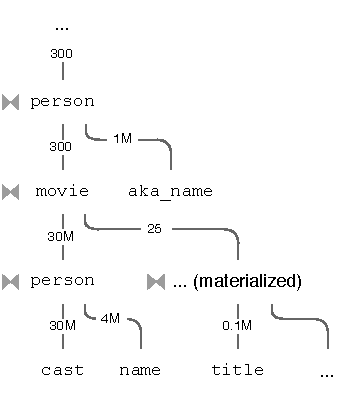
\includegraphics[width=0.7\linewidth]{q56-plan.pdf}
  \caption{
    Fragment of query plan produced by DuckDB.
    The number after each operation counts the output tuples.
  }
  \label{fig:q56-plan}
\end{figure}

Despite the guarantees on asymptotic complexity,
  Mhedhbi and Salihoglu~\cite{} 
  and Freitag et.al.~\cite{} 
  have 
  % \ds{Who has observed that?}
 observed that \GJ can be slow in practice.
Its inefficiency can be demonstrated by the following query fragment\footnote{Simplified for clarity.}
  from the Join Order Benchmark~\cite{DBLP:journals/pvldb/LeisGMBK015}:
%
 \begin{lstlisting}[
   language=SQL,
   showspaces=false,
   basicstyle=\ttfamily\small,
   numbers=left,
   numberstyle=\tiny,
   commentstyle=\color{gray},
   deletekeywords={CAST}
]
SELECT ...
  FROM cast, name, title, aka_name, ... 
 WHERE cast.person = name.person
   AND cast.movie = title.movie
   AND cast.person = aka_name.person
   AND ...
\end{lstlisting}
%
A fragment of the query plan (using binary hash joins) produced by DuckDB 
  is shown in Figure~\ref{fig:q56-plan}.
The first notable detail is the large size of the \texttt{cast} relation.
Since \texttt{cast} is on the left, 
  the binary join simply iterates over each tuple in the relation.
In contrast, \GJ would build a hash table for \texttt{cast},
  which is very expensive.
Here we make a simple yet powerful observation:
  \GJ can simply iterate over certain relations
  instead of building hash tables for them.
In other words, \textbf{we only need to build a hash table 
  for a relation before we probe into it}.
This avoids the cost of building large hash tables, 
  which in our experiments can take much longer 
  than the run time of the entire query.
This example demonstrates the general principle 
  to build hash \emph{lazily}, 
  which is the central idea behind our \COLT data structure.

Another source of inefficiency lies in the main loop of \GJ. 
Looking back at the join plan,
  we see that the first and third joins are not selective,
  while the second join is very selective.
Following this plan, the first two binary joins require
  30 million lookups each, 
  and the third join requires 300 lookups.
In total this sums to a just over 60 million lookups.
\GJ, on the other hand, joins all three relations on \texttt{person}
  at the same time, before the selective join on \texttt{movie}.
This means the join on \texttt{person} incurs 30 million lookups
  each on \texttt{name} and \texttt{aka\_name},
  and the join on \texttt{movie} incurs yet another 30 million lookups.
In total, \GJ performs 90 million lookups.

The root cause of \GJ's inefficiency is that it insists on 
  joining \emph{all} relations involving the same variable at the same time.
Our remedy is to simply relax this requirement,
  delaying certain relations to be joined later.
We call this optimization \textbf{variable splitting}.
In this example, we split the three-way join on \texttt{person}
  into a join between \texttt{cast} and \texttt{name},
  and delay the join on \texttt{aka} 
  until after joining on \texttt{movie}.
By doing so, we recover exactly the original binary plan.

There is another way to improve the performance of \GJ.
Instead of splitting the join on \texttt{person}, 
  we \emph{merge} the joins on \texttt{movie} and \texttt{person}.
Although the original \GJ algorithm can only join on one variable at a time,
  since we iterate over each tuple in \texttt{cast},
  we can join on \texttt{movie} and \texttt{person} at the same time.
In particular, while iterating over \texttt{cast} we may 
  dynamically decide which one of \texttt{name}, \texttt{aka\_name}, 
  and \texttt{title} to probe first.
In this example, it turns out the materialized intermediate
  only contains 25 tuples. 
\GJ can take this runtime information into account
  and prioritize probing the materialized intermediate.
We call this optimization \textbf{variable merging}
  which captures and generalizes classic multiway join algorithms
  like Hash Teams~\cite{} and Eddies~\cite{}.

Variable splitting and merging chart a design space of join algorithms
  that covers both binary join and \GJ, 
  as well as traditional multiway joins.
We illustrate this design space in Figure~\ref{fig:free-join}.
Each point in the design space can be derived by specifying 
  how many variables to join on, 
  as well as how many relations involving those variables to join on.
\textbf{
Being able to join on any number of variables and relations
  frees us from the constraints of existing algorithms.
}
Thereby we unify existing algorithms into a new, 
  general framework called \FJ.

% Through the lens of \FJ, we shall see that binary join and \GJ 
%   are not so different after all.
% In fact, we will show that many of the key techniques
%   that are considered staples of traditional join algorithms 
%   can also be applied to \FJ in a straightforward way.
% Specifically, we propose:
% %
% \begin{itemize}
%   \item \COLT (for \emph{Column-Oriented Lazy Trie}), a column-oriented trie data structure for \FJ
%   \item A vectorized execution algorithm for \FJ 
%   \item An algorithm to convert any binary join plan to a \FJ plan 
%     that runs as fast or faster
% \end{itemize}
% %
% We hope practitioners will find the final point particularly appealing: 
%   it allows them to reuse the existing query optimizer
%   and implement \FJ as a drop-in replacement for binary join.

% In summary, we make the following contributions in this paper:
% \begin{enumerate}
%   \item \FJ, a framework unifying existing join algorithms
%   \item Optimizations to split and merge variables that 
%     improve the performance of \FJ beyond existing algorithms
%   \item Techniques to adapt column-oriented layout, vectorization and query optimization
%     to further speed up \FJ
%   \item A proof that the run time of \GJ is asymptotically bounded by that of binary join
%     on any query and database
%   \item Experiments evaluating the algorithms and optimizations
% \end{enumerate}

\section{Scratch}
\begin{itemize}
  \item A figure showing join plans for binary join, \GJ, and \FJ. 
  \item Index join example.
  \item Architecture diagram.
  \item Column-wise layout.
  \item Benchmarks.
  \item TACO?
\end{itemize}


\subsection{Analysis of Asymptotic Run Time}
\begin{definition}[Left-deep Linear Plan]
  A left-deep linear plan is a sequence of relations. 
  The first relation is called the ``left'' relation.
  Every relation in the sequence joins with all previous
    relations on all common variables.
\end{definition}

\begin{definition}[Step-wise Plan]
  Given a left-deep linear plan, 
    we derive its step-wise plan by expanding
    each join involving more than one variable.
  For each join involving variables $x_1, \ldots, x_n$,
    we replace it with $n-1$ left-semijoins,
    each one on $x_1, \ldots, x_i$ for $i = 1, \ldots, n$,
    followed by the original join.
\end{definition}

\begin{lemma}
  Given a left-deep linear plan running in time $T(I)$
    where $I$ is a database instance,
    its step-wise plan runs in time $O(T(I))$.
\end{lemma}
\begin{proof}
  Each join operation in the left-deep linear plan is replaced
    by a constant number of semijoins plus one natural join
    in the step-wise plan.
  Each semijoin runs in time linear in the run time of the original join,
    and the run time of the final natural join in the step-wise plan
    is also bounded by the run time of the original join.
  Therefore, the total run time of the step-wise plan is linear
    in the run time of the left-deep linear plan.
\end{proof}

\begin{theorem}
  Fix a database $I$. 
  For any binary join plan that runs in time $T(I)$,
   there exists a generic join plan that runs in time $O(T(I))$.
\end{theorem}
\begin{proof}
  We first generate a variable ordering from the binary join plan.
  Given a left-deep linear plan, 
    we generate a variable ordering by traversing the plan bottom-up,
    adding each new variable to the ordering if it has not been added yet.
  If a binary join involves more than 1 variable,
    we visit them in the order they appear in the join.

  Expand the binary plan into a step-wise plan.
  We now prove that \GJ with the variable ordering
    specified above runs in time linear in the run time of the step-wise plan,
    which is linear in the run time of the binary plan.

  Now consider for a given $i$, 
    the $i$-th \GJ loop together with the $i$-th step-wise join.
  Let $l_i$ be the number of iterations of the $i$-th \GJ loop,
    and $t_i$ be the number of tuples arriving at the $i$-th binary join.
  Let $x_1, \ldots, x_{i-1}$ be the first $i-1$ variables in the ordering.
  Then we have: 
%
\begin{align}
    & = t_i
\end{align}
%
  Here we use a few ad-hoc notations to reduce clutter:
  \begin{itemize}
    \item $(x_1 : v_1, x_2 : v_2, \ldots)$ is a tuple where variable $x_a$ has value $v_a$.
    \item $R_j(x_a, x_b, \ldots)$ means some variables $x_a, x_b$ from the tuple appears in the relation $R_j$.
    \item $(v_a, v_b) \in R_j$ means $R_j$ contains a tuple where $x_a = v_a$ and $x_b = v_b$.
  \end{itemize}
  In other words, the set in Equation~\ref{eq:gj-vs-bj:gj} contains only tuples that appear in the join of \emph{all}
    relations that contain variables $x_1, \ldots, x_{i-1}$,
    whereas the set in Equation~\ref{eq:gj-vs-bj:bj} contains tuples that appear in the join of the first $i$ relations
    in the step-wise plan.
\end{proof}

% R(x, y), S(y, z), T(x, z)
\begin{lstlisting}[mathescape=true]
  X = R.x $\cap$ T.x
  for x in X
    Y = R[x].y $\cap$ S.y
    for y in Y
      Z = S[y].z $\cap$ T[x].z
      for z in Z
        yield (x, y, z)
\end{lstlisting}


\subsection{Analysis of absolute run time}
Before we formally analyze the run time of \FJ,
  let us gain some intuition of why \FJ can run faster than binary join.
\begin{example}
  Consider again the ``sand dollar'' query: 
%
  $$Q(x, a, b, c) \cd R(x, a), S(x, b), T(x, c).$$
%
  The plans are nearly identical, 
   except that the free join plan hoists the lookup on $T$ out of the second loop.
  This means that the free join plan makes fewer lookups on $T$.
  Moreover, the middle loop over $b$ in $S$ is also invoked fewer times, 
   since the lookup on $T$ may fail and continue to the next iteration of the outer loop.
\end{example}

With this intuition, we can now prove the absolute run time of \FJ
  is bounded by that of the corresponding binary join plan.

\begin{theorem}
  Fix a database $I$. 
  For any binary join plan that runs in time $T(I)$,
   there is a free join plan that runs in time \emph{at most} $T(I)$.
\end{theorem}
%
\begin{proof}
  We convert a binary join plan into a free join plan 
    by hoisting lookups whenever possible.
  Each successful hoist strictly reduces run time, 
    since it reduces the number of calls to the hoisted lookup
    and also the number of invocations of the hoisted loop.
  Note that the transformed plan still uses the exact same hash tables
    as the original binary plan, 
    so the cost of hash building remains unchanged.
  Therefore, the resulting free join plan must be as efficient 
    as the original binary join plan.
\end{proof}

\begin{enumerate}
  \item Asymptotic proof.
  \item Q056 analysis.
  \item Iteration trick (show cost of trie construction).
  \item Variable splitting and merging.
  \item Light and heavy tries with degree constraints.
  \item Exact cost proof.
\end{enumerate}

\begin{itemize}
  \item Degree distribution.
  \item Cost of hash building compared to total cost.
  \item Na\"ive GJ run time.
  \item Effect of iteration.
  \item Effect of variable splitting.
  \item Effect of variable merging.
  \item Robustness against bad plan.
\end{itemize}